%%%%%%%%%%%%%%%%%%%%%%%%%%%%%%%%%%%%%%%%%%%%%%%%%%%%%%%%%%%%%%%%%
\subsubsection{Theorem 28}		%	TESTFÄLLE - RMed - Theorem 28
%%%%%%%%%%%%%%%%%%%%%%%%%%%%%%%%%%%%%%%%%%%%%%%%%%%%%%%%%%%%%%%%%

\noindent
Nach Theorem~\ref{theo: med_28} des Papers~\cite{meyer2} erreicht das Median Element für $k(n)=n^{2/3}$ und $d(n)=n^{1/12}$ eine erwartete \fg von $\mathbb{E}[f_{med}(n)]=\mO(\log\log(n))$ und alle übrigen Elemente $\mathbb{E}[f_{rem}(n)]=\mO(\sqrt{n})$.\\[.1cm]





\subsubsection*{\textit{Fragile complexity} des Median Elements}
Zuerst wird die \fg des Medians \fgM untersucht. Wie bereits erwähnt findet ein die Werte verzerrender Sprung statt, wie in Abbildung~\ref{fig: med_theo28_work} deutlich zu sehen. Die Arbeit $w(n)$ verhält sich jedoch wie erwartet linear, was Theorem~\ref{theo: med_30} bestätigt.

%---------------------------------------------------------------
%	FIG: FG COMP
\begin{figure}[H]
	\hspace*{-.6cm}
    \begin{minipage}[t]{.30\textwidth}
        \centering
		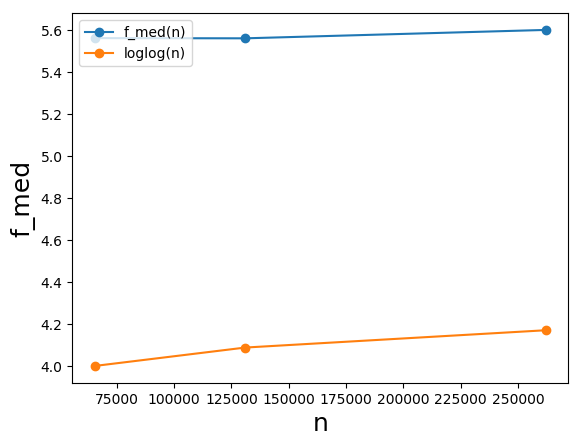
\includegraphics[width=\textwidth]{pictures/med_algo_theo28_med}
    \end{minipage}
    \hspace*{.4cm}
    \begin{minipage}[t]{.30\textwidth}
        \centering
        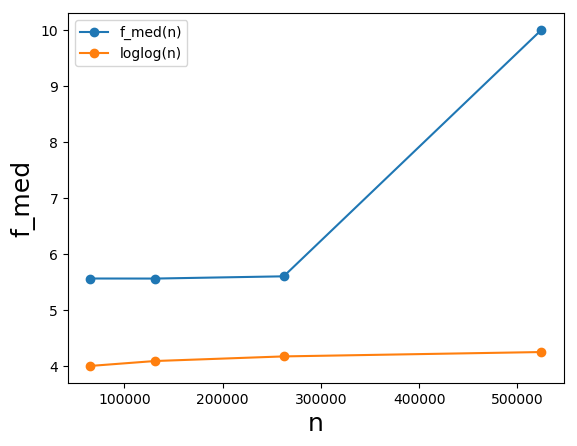
\includegraphics[width=\textwidth]{pictures/med_algo_theo28_med_jump}
    \end{minipage}
    \hspace*{.4cm}
    \begin{minipage}[t]{.30\textwidth}
        \centering
        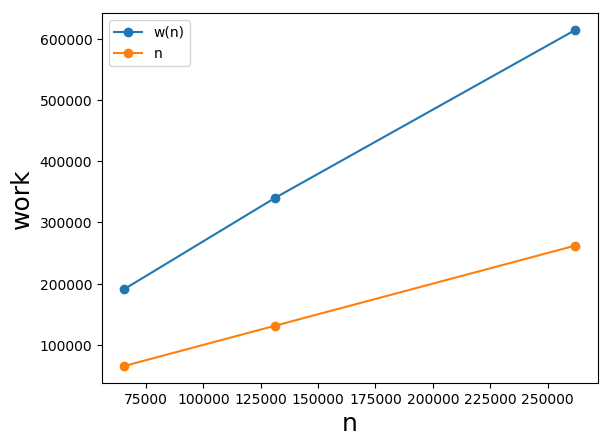
\includegraphics[width=\textwidth]{pictures/med_algo_theo28_work.png}
    \end{minipage}
    \vspace*{-0.1cm}
    \captionof{figure}{$\log(n)=16,\cdots,18$ gegenüber $\log(n)=16,\cdots,19$ sowie die Arbeit $w(n)$.}\label{fig: med_theo28_work}
\end{figure}


%---------------------------------------------------------------
\noindent
Auch wenn die Datenmenge sowie der gesammelte Bereich nicht ausreichen, um eine feste Aussage zu tätigen, wurde die \fg trotzdem für $\log(n)=16,\cdots,18$ untersucht. Die Daten wurden hierbei wieder gegen einen einfach-logarithmischen mit $F^1(n)=a\cdot\log(n) + b$ sowie eine doppelt-logarithmischen Term $F^2(n)=a\cdot\log\log(n) + b$ abgeglichen.

\begin{center}
\begin{tabular}{c||l|l|l|l}

&\multicolumn{1}{c|}{Param $a$}&
\multicolumn{1}{c|}{Param $b$}&
\multicolumn{1}{c|}{Sum Res}&
\multicolumn{1}{c}{$\Delta$ Last Iter}\\
\hline
$F^1(n)$:&$0.2272$&$4.6452$&$0.0002$&$-2.42876e-07$\\
\hline
$F^2(n)$:&$0.0195$&$5.2419$&$0.0002$&$-1.9372e-14
$
\end{tabular}
\end{center}
Die sich ergebenden experimentellen Daten sowie ihre grafische Veranschaulichung in Abbildung~\ref{fig: med_theo28_med} deuten stark auf einen, wie von Theorem~\ref{theo: med_28} angegebenen, doppelt-logarithmischen Zusammenhang hin. Eine logarithmische Achsenskalierung hilft hier jedoch nicht, um eine Abschätzung jeglicher Form zu unterstützen. 


%---------------------------------------------------------------
%	FIG: FG COMP
\begin{figure}[H]
	\hspace*{-0.4cm}
    \begin{minipage}[t]{.30\textwidth}
        \centering
		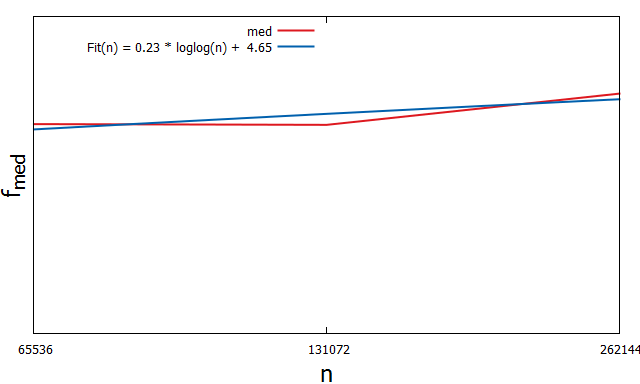
\includegraphics[width=1.15\textwidth]{pictures/med_algo_theo28_fit_med_loglog}
    \end{minipage}
    \hspace*{.6cm}
    \begin{minipage}[t]{.30\textwidth}
        \centering
        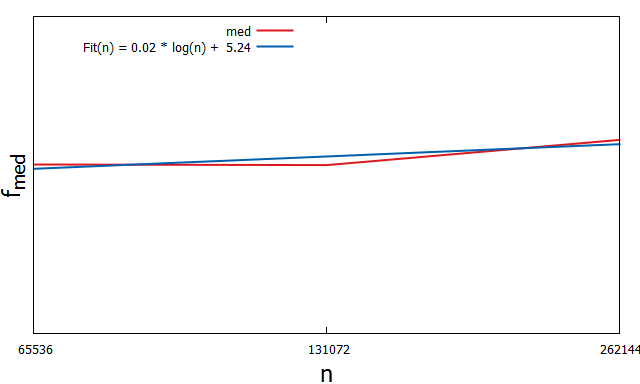
\includegraphics[width=1.15\textwidth]{pictures/med_algo_theo28_fit_med_log}
    \end{minipage}
    \hspace*{.8cm}
    \begin{minipage}[t]{.30\textwidth}
        \centering
        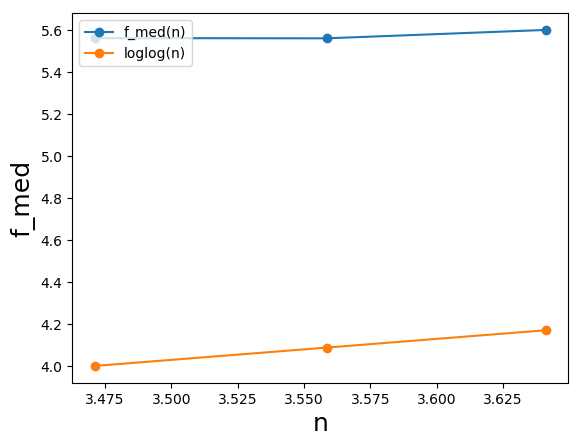
\includegraphics[width=\textwidth]{pictures/med_algo_theo28_med_logscale.png}
    \end{minipage}
    \vspace*{-0.1cm}
    \captionof{figure}{$\log$ vs $\log\log$ Fit sowie logarithmische Achsenskalierung.}\label{fig: med_theo28_med}
\end{figure}


%---------------------------------------------------------------
\noindent

\subsubsection*{\textit{Fragile complexity} aller nicht-Median Elemente}
Für die \fg aller nicht-Median Elemente \fgr hingegen konnte eine aussagekräftige Regression gewonnen werden.\\[.05cm]
Wie in Abbildung~\ref{fig: med_theo28_rem} zu sehen wurde hier ein Fit der Form $F(n)= a \cdot \sqrt{n} + b$ mit einer Parametrisierung von $a=2.3374$  $b=-155.424$ bestimmt.


%---------------------------------------------------------------
%	FIG: FG COMP
\begin{figure}[H]
	\hspace*{-.8cm}
    \begin{minipage}[t]{.30\textwidth}
        \centering
		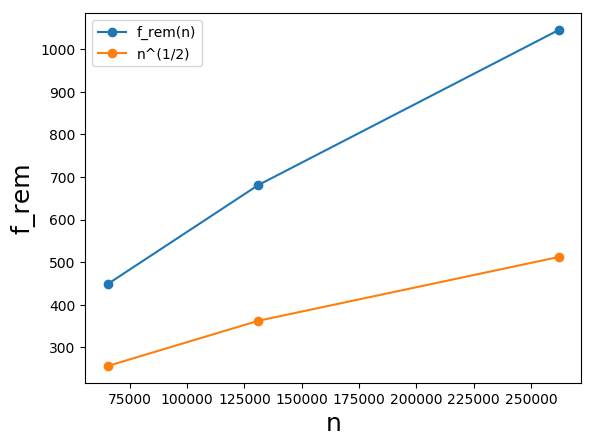
\includegraphics[width=\textwidth]{pictures/med_algo_theo28_rem}
    \end{minipage}
    \hspace*{.3cm}
    \begin{minipage}[t]{.30\textwidth}
        \centering
        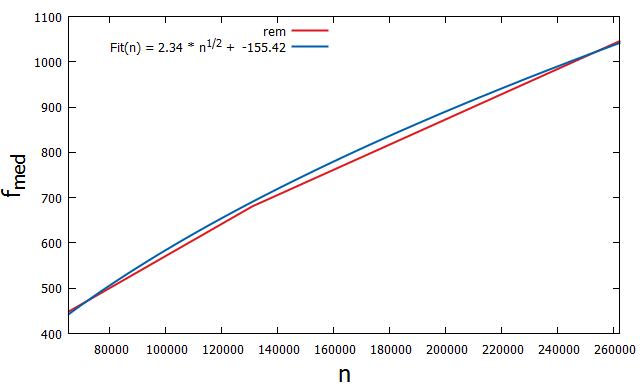
\includegraphics[width=1.25\textwidth]{pictures/med_algo_theo28_fit_rem}
    \end{minipage}
    \hspace*{1.2cm}
    \begin{minipage}[t]{.30\textwidth}
        \centering
        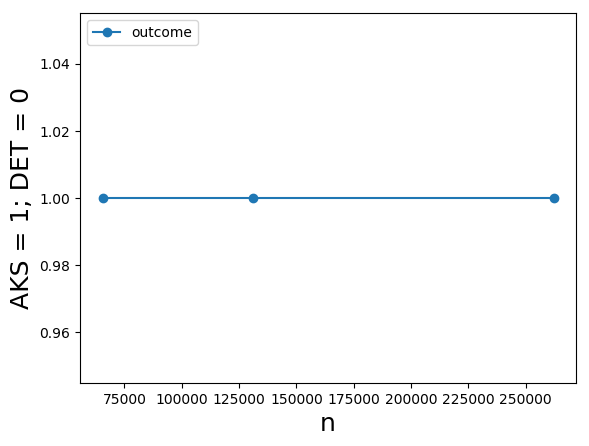
\includegraphics[width=\textwidth]{pictures/med_algo_theo28_case.png}
    \end{minipage}
    \vspace*{-0.1cm}
    \captionof{figure}{Vorhersage und Fit für \fgr sowie der Ausgang von Phase 3.}\label{fig: med_theo28_rem}
\end{figure}


%---------------------------------------------------------------
\noindent
Abschließend sei hier noch angemerkt, dass bei allen für die Grafiken genutzten Experimentaldaten der Algorithmus \RM mit der Ausführung des \textit{AKS}-Algorithmus endet.




